\chapter{Divide-and-Conquer Lexer}
An incremental divide and conquer lexer works by dividing the sequence, to be lexicaly analysed,
into small parts and analyse them; and then combining them. In the base
case the lexical analysis is done on a single character. The conquer step
then combines the smaller tokens into as large tokens as possible. The end
result is a sequence of token that represent the code. How this is done
will be described below.

\section{Divide and Conquer in General}
This section gives an idea of how the Divide and Conquer algorithm
works in general, before adressing in detail how to apply it to lexing.
% So when talking about the incremental lexer there is an understanding about the underlying techniques.

\subsection{The Three Steps}
The general idea of a divide and conquer algorithm is to divide a problem into
smaller parts, solve them indepently and then combine the results. A Divide
and Conquer algorithm always consists of a pattern with these three steps \cite{Goodrich}.
\begin{description}
\item[Divide:] If the input size is bigger than the base case then divide the
input into subproblems. Otherwise solve the problem using a straightforward
method.
\item[Recur:] Recursively solve the subproblems associated with the subset.
\item[Conquer:] Given the solutions to the subproblems, combine the results to
solve the original problem.
\end{description}

\subsection{Associative Function}
An associative function, or operator, is a function that doesn't care in what
order it is applied. An example of such a function is $+$, which is associative
since it has the propert in \cref{assprop}.

In divide and conquer algorithms this is essential. In the divide step of the
divide and conquer algorithm, there is no certain order of how the subproblems
are going to be divided. This means that the order the subproblems are being
conquered can't have an impact on the algorithm, hence the conquer step must be
associative.

\begin{example}[Associativity of the conquer step]\label{assprop}
Let $f(x,y)$ be the conquer function, where $x$ and $y$ are of the same type as
the result of $f$, then:
\begin{center}
$f(x,f(y,z)) = f(f(x,y),z)$
\end{center}
Otherwise the algorithm can give different results for the same data.
\end{example}

\subsection{Time Complexity}
To calculate the running time of any divide and conquer algorithm the master
method can be applied \cite{Cormen}. This method is based on the following
theorem.
\begin{theorem}[Master Theorem \cite{Cormen} \label{MasterTheo}] $ $\\
Assume a function $T_n$ constrained by the recurrence
\begin{center}
$T_n = {\alpha}T_{\frac{n}{\beta}}+ f(n)$
\end{center}
(This is typically the equation for the running time of a divide and conquer algorithm, where $\alpha$
is the number of sub-problems at each recursive step, $n/\beta$ is the size of
each sub-problem, and $f(n)$ is the running time of dividing up the problem
space into $\alpha$ parts, and combining the sub-results together.)\\
If we let $e = log_\beta \alpha$, then
\begin{center}
\begin{tabular}{r c l l}
1. $Tn$ & $=$ & $\Theta(n^{e})$ &  if $f(n) = O(n^{e - \epsilon})$ and $\epsilon > 0$\\
2. $Tn$ & $=$ & $\Theta(n^{e} log n)$ & if $f(n) = \Theta(n^e)$\\
3. $Tn$ & $=$ & $\Theta(f(n))$ & \begin{minipage}[t]{0.6 \columnwidth}
  if $f(n) = \Omega(n^{e+\epsilon})$ and $\epsilon > 0$
  and $\alpha \cdot f(n/\beta) \leq c \cdot f(n)$
  where $c < 1$ and all sufficiently large $n$
  \end{minipage}
\end{tabular}
\end{center}
\qeda
\end{theorem}

\subsection{Hands on Example}
The divide and conquer pattern can be preformed on different sorts of algorithm
that solves different problems. A general problem is sorting, or more precisely
sorting a sequence of integers. This example shows merge-sort.

\begin{description}
\item[divide:] The algorthim starts with the divide step. Given the input $S$ the algorithm
will check if the length of $S$ is less then or equal to 1.
\begin{itemize}
\item If this is true, the sequence is returned. A sequence of one or zero
elements is always sorted.
\item If this is false, the sequence is split into two equaly big sequences,
$S_1$ and $S_2$. $S_1$ will be the first half of $S$ while $S_2$ will be the
second half.
\end{itemize}
\item[Recur:] The next step is to sort the subsequences $S_1$ and $S_2$. The sorting
function sorts the subsequences by recursivly calling itself twice with $S_1$ and
$S_2$ as arguments respectivly.
\item[Conquer:] Since $S_1$ and $S_2$ are sorted combining them into one sorted
sequence is trivial. This process is what's refered to as merge in merge-sort.
The resulting sequence of the merge is returned.
\end{description}
Algortihm~\ref{Alg:MergSort} shows a more formal definition of merge-sort.

\begin{algorithm}
\DontPrintSemicolon
\KwData{Sequence of integers $S$ containing $n$ integers}
\KwResult{Sorted sequence $S$}
\If {$length(S) \leq 1$}{
  \Return $S$ \;
}
\Else {
  $(S_1,S_2) \gets splitAt(S,n/2)$ \;
  $S_1 \gets MergeSort(S_1)$\;
  $S_2 \gets MergeSort(S_2)$\;
  $S \gets Merge(S_1, S_2)$\;
  \Return $S$
}
\caption{MergeSort}
\label{Alg:MergSort}
\end{algorithm}

Given the mergesort algorithm, time complexity can be calculated as follows
using the master method. There are $2$ recursive calls and the subproblems are
$1/2$ of the original problem size, so $\alpha=2$ and $\beta=2$. To merge the
two sorted subproblems the worst case is to check every element in the two list,
$f(n) = 2 \cdot n/2 = n$.
\begin{center}
$T(n) = 2T(n/2) + n$\\
$e=log_\beta\alpha=log_22=1$
\end{center}
Case 2 of the master theorem applies, since
\begin{center}
$f(n) = O(n)$
\end{center}
So the solution will be:
\begin{center}
$T(n) = \Theta(n^{log_2 2} \cdot log n) = \Theta(n \cdot log n)$
\end{center}

\section{Fingertree}
A smart lexer needs smart structures to save its data. This section describes 
the tree structure of a FingerTree.

\subsection{Fundamental Concepts}
Before describing the functionality, lets take a look on which building blocks
the fingertrees uses.
\paragraph{First,}
fingertrees uses monoids which in abstract algebra is a set, $S$, and a binary operation $\bullet$ which fulfills the following
three properties:
\begin{description}
\item[Closure] $\forall a,b \in S: a \bullet b \in S$
\item[Associativity] $\forall a,b,c \in S: (a \bullet b) \bullet c = a \bullet (b \bullet c)$
\item[Identity element] $\exists e \in S: \forall a \in S: e \bullet a = a \bullet e = a$
\end{description}

\paragraph{Second,} 
fingertrees uses Right and Left Reductions. This is a function which
collapses a structure of $f$ $a$ into a single value of type $a$. The base case
for when the tree is empty is replaced with a constant value, such as 
$\emptyset$. Intermediate results are combined using a binary operation, like
the monoids $\bullet$. Reduction with a monoid always return the same value,
independent of the argument nesting. But for a reduction with an arbitrary
constant and binary operation there must be a specified nesting rule. If
combining operation are only nested to the right, or to the left, the obtained
result will be a skewed reductions, which can be singled out as a type class.
\lstinputlisting[language=Haskell]{examples/FingerTreeReduceFun.hs}

\subsection{Simple Sequence}
lets take a look on the definition on a 2-3 fingertree and how they can
implement a sequence. Lets start by looking at an ordinary 2-3 tree like in \cref{fig:2-3tree}.
\begin{figure}[!h]
  \centering
\tikzset{
  treenode/.style = {align=center, inner sep=0pt, text centered,
    font=\sffamily},
  branch/.style = {treenode, circle, draw=black, minimum size=0.2cm, text width=0.2em},
  leaf/.style = {treenode, circle, draw=black, font=\sffamily\bfseries, text width=1.5em}
}
    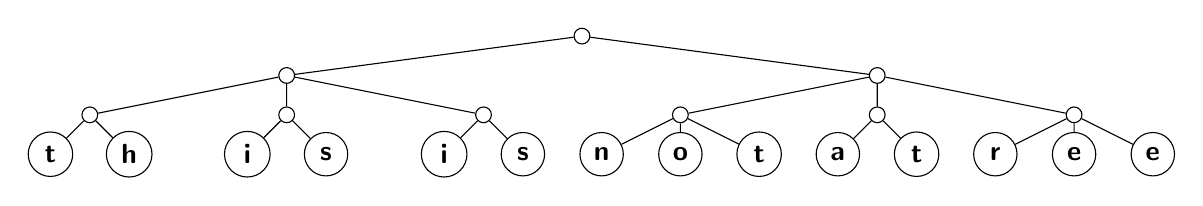
\begin{tikzpicture}[auto,
                        level 1/.style={sibling distance=7.5cm},
                        level 2/.style={sibling distance=2.5cm}, 
                        level 3/.style={sibling distance=1cm},
                        level distance = 0.5cm] 
\node [branch] {}
    child{ node [branch] {}
        child{ node [branch] {}
        	child{ node [leaf] {t}
            }
			child{ node [leaf] {h}
            }
        }
        child{ node [branch] {}
        	child{ node [leaf] {i}
            }
			child{ node [leaf] {s}
            }
        }
        child{ node [branch] {} 
        	child{ node [leaf] {i}
            }
			child{ node [leaf] {s}
            }
        }
    }
    child{ node [branch] {}
        child{ node [branch] {} 
        	child{ node [leaf] {n}
            }
			child{ node [leaf] {o}
            }
			child{ node [leaf] {t}
            }
        }
        child{ node [branch] {} 
        	child{ node [leaf] {a}
            }
			child{ node [leaf] {t}
            }
        }
        child{ node [branch] {} 
        	child{ node [leaf] {r}
            }	
			child{ node [leaf] {e}
            }
			child{ node [leaf] {e}
            }
        } 
    }
; 
\end{tikzpicture}
  \caption{Ordinary 2-3 tree
  \label{fig:2-3tree}}
\end{figure}
In this section the tree will store all data in the leafs. This can be expressed
by defining an non-regular or nested type, as follows:
\lstinputlisting[language=Haskell]{examples/FingerTree2-3Tree.hs}
Operations on these types of trees usually takes logarithmic time in the size of
the tree. But for sequence representations a constant time complexity is
preferable for adding or removing element from the start or end of the sequence.

A finger is a structure which provides efficient access to nodes near the
distinguished location. To obtain efficient access to the start and end of the
sequence represented by the tree, there should be fingers placed at the left and
right end of the tree. In the example tree, taking hold of the end nodes of and
lifting them up together. The result should look like in \cref{fig:fingertree}
\begin{figure}[!h]
  \centering
  \tikzset{
  treenode/.style = {align=center, inner sep=0pt, text centered,
    font=\sffamily},
  branch/.style = {treenode, circle, draw=black, minimum size=0.2cm, text width=0.2em},
  blackbranch/.style = {treenode, draw,fill=black!33, minimum size=0.2cm, text width=0.2em},
  leaf/.style = {treenode, circle, draw=black, font=\sffamily\bfseries, text width=1.5em}
}
    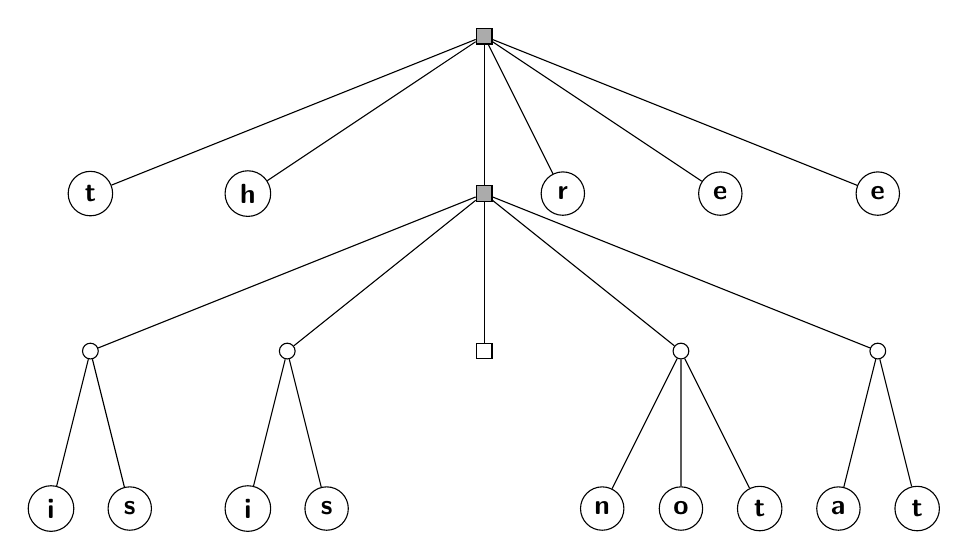
\begin{tikzpicture}[level distance=2cm, sibling distance = 2cm]
    \node[blackbranch] {} 
        child { node[leaf] {t} }
        child { node[leaf] {h} }
        child[level distance=2cm, sibling distance=2.5cm, grow=down] { node[blackbranch] {} [level distance=2cm]
            child { node[branch] {} [sibling distance=1cm]
                child { node[leaf] {i} }
                child { node[leaf] {s} }
            }            
            child { node[branch] {} [sibling distance=1cm]
                child { node[leaf] {i} }
                child { node[leaf] {s} }
            }
            child[level distance=2cm, grow=down] { node[blackbranch, fill=white] {}}
            child { node[branch] {} [sibling distance=1cm]
                child { node[leaf] {n} }
                child { node[leaf] {o} }
                child { node[leaf] {t} }
            }
            child { node[branch] {} [sibling distance=1cm]
                child { node[leaf] {a} }
                child { node[leaf] {t} }
            }
        }
        child { node[leaf] {r} }
        child { node[leaf] {e} }
        child { node[leaf] {e} }
    ;
  \end{tikzpicture} 
  \caption{2-3 Fingertree
  \label{fig:fingertree}}
\end{figure}

Since all leafs in the 2-3 tree where at the same level, the left and right
spine has the same length. Therefor the left and right spines can be pair up to
create a single central spine. Branching out from the spine is 2-3 trees. At the
top level there are two to three elements on each side, while the other levels
have one or two sub-trees, whose depth increases down the spine. Depending on if
the root node had 2 or 3 branches in the original 2-3 tree, will the bottom node
either have a single 2-3 tree or empty. This structure can be described as
follows:
\lstinputlisting[language=Haskell]{examples/HaskellFingerTree.hs}
Where Digit is a buffer of elements stored left to right, here represented as a
list for simplicity

The non-regular definition of the $FingerTree$ type determines the unusual shape
of these trees, which is the key to there performance. The top level of the tree
contains elements of type $a$. Next level contains elements of type $Node$ $a$.
At the $n$th level, elements are of type $Node^n$ $a$. which are 2-3 trees with
a depth of $n$. This will give that a sequence of $n$ elements is represented by
a $FingerTree$ of depth $\Theta(\log n)$. Also an element at position $d$ from
the nearest end is stored at a depth of $\Theta(\log d)$ in the $FingerTree$
\cite{fingertree}

In fingertrees and nodes the reduce function mentioned in fundamental concepts
will be generic defined to the following types. 
Reduction for the node:
\lstinputlisting[language=Haskell]{examples/FingerTreeReduceNode.hs}
Reduction of fingertrees single and double lifting of the binary operation:
\lstinputlisting[language=Haskell]{examples/FingerTreeReduceFingerTree.hs}

\subsection{Double-ended Queue Operations}
After showing how the Fingertrees basic structure is defined. It is now time to
show how fingertrees makes efficient Double-ended Queue, a queue structure which
can be accessed from both ends, where all operations having the time complexity
$\Theta(1)$.

Adding a element to the beginning of the sequence is strait forward, except when
the initial buffer ($Digit$) already is full. In this case, push all but one of
the elements in the buffer as a node, leaving behind two elements in the buffer:
\lstinputlisting[language=Haskell]{examples/FingerTreeInfixr.hs}
Adding to the end of the sequence is a mirror image of the above:
\lstinputlisting[language=Haskell]{examples/FingerTreeInfixl.hs}

A insertion operation the basic 2-3 tree, where the data is stored in the leafs,
is done with a time complexity of $\Theta \log n$. In the fingertree the
expected time complexity can be argued in the following way. Digits of two or
three elements (which is isomorphic to elements of type $Node$ $a$) is
classified as safe and those of one or four elements is classified as dangerous.
A double-ended queue operation can only propagate to the next level from a
dangerous element. By doing so making that dangerous element safe, which means
that the next operation reaching that digit will not propagate. This will result
in that at most half of the operations descend one level, at most 1 quarter two
levels, and so on. This will give that in a sequence of operations the average
cost is constant.

The same bound hold in a persisted setting if subtrees are suspended using lazy
evaluation. Laziness makes sure that changes deep in the spine do not take place
until a subsequent operation need to go that far. By the above properties
of safe and dangerous digits, by that time enough cheap shallow operations
will have been performed to pay for the more expensive operation \cite{fingertree}.

\subsection{Concatenation Operations}
Concatenation is a simple operation for most cases, except for the case when two $Deep$ trees are being concatenated. Concatenating with a $Empty$ will be an identity and with a $Single$ will reduce to $<|$ or $|>$. For the hard part when there are two $Deep$ trees, the prefix of the first tree will be the final prefix. Suffix of the second tree will be the suffix of the final tree. The recursive function $app3$ combines two trees and a list of $Nodes$ (basically the old prefix and suffixes down the spines of the old trees):

\lstinputlisting[language=Haskell]{examples/FingerTreeApp3.hs}

Where $(<|')$ and $(|>')$ are the functions defined in the previous sub-section and $nodes$ groups a list of elements into $Node$s: 

\lstinputlisting[language=Haskell]{examples/FingerTreeNodesFunc.hs}

Now to concatenation of the Fingertrees, just call on $app3$ with an empty list between the two trees.

\lstinputlisting[language=Haskell]{examples/FingerTreeConcatFunc.hs}

The time spent on concatenation can be reasoned in this way. Each invocation of $app3$ arising from $(><)$ the argument list has a length of at most 4, which means that each of these invocations takes $\Theta(1)$ time. The recursion terminates when the bottom of the shallower tree has been reached, with up to 4 insertions. So the total time complexity id $\Theta(\log min\{n_1, n_2\})$ where $n_1$ and $n_2$ are the number of elements in the two trees. 

\section{Divide and Conquer Lexing in General}
In the last section we covered the general divide and conquer algorithm. This
section covers the general data structures and algorithms for an incremental
divide and conquer lexer.

\subsection{Treestructure} % work in progress.
The incremental divide and conquer lexer should use a structuer where the
code-lexemes can be related to its tokens, current result can be saved and easy
recalculated. A divide and conquer lexer should therefore use a tree structure
to save the lexed result in. Since every problem can be divided in to several
subproblems, until the basecase is reached. This is cleraly a tree structure of
solutions, where a leaf is a token for a single character. and the root
is a sequence of all tokens in the code.  


%TODO master thereom

\subsection{Transition map} % before treestructure?
When storing a result of a lexed string it is a good idea to store more then
just the tokens. In particular the in and out states are needed when combining
the lexed string with another string. We will henceforth refer to this as a
$transition$.
\begin{verbatim}
type Transition = (State,[Token],State)
\end{verbatim}
Since the lexer doesn't know if the current string is a prefix of the entire
code or not it can't make any assumptions on the in state. Because of this the
lexer needs to store a transition for every possible in state, we will henceforth
refer to this as a \emph{transition map}.
\begin{verbatim}
type Transition_map = [Transition]
\end{verbatim}
\paragraph{The Base Case}
When the lexer tries to lex one character it will create a transition
map using the DFA for the language. It will for each state create a transition
that has the state as in state, a list containing the character as the only
token and by using the DFA, lookup what out state the transition should have.
For the character '/' part of a transition map might look like the following.

In the
examples below the first number refers to the in state, the middle part is the
sequence of tokens and the second number is the out state, that can be accepting.
\begin{center}
$\left[\begin{array}{ccc}
10&Single '/'&10\\
11&Single '/'&NoState\\
12&Single '/'&10\\
\end{array}\right]$
\end{center}
$NoState$ transition is used to tell the lexer that using that particular 
transition will result in a lexical error. For reasons being covered in
\cref{longmatch}, they can't be discarded.

\paragraph{Conquer Step}
The conquer step of the algorithm is to combine two transition maps in to one
transition map. This is done by, for every transtion in the left transition map, combining
the transition with the transition in the right transition map that has the same in state as the
left transitions out state. This can be described byt the following logical statement where $T_1$ and $T_2$ refers to the first and second transition map.
\begin{center}
$\forall.t_1\in T_1\;\exists.t_2\in T_2\;o_1=i_2,o_1=outState(t_1),i_2=inState(t_2)
\vdash t_{new}=merge(t_1,t_2)$
\end{center}

The most general case is a naive lexer that takes the first accepting state it
can find. When two transitions are combined there are two different outcomes:
\begin{description} 
  \item[Concat:]If the out state of the first transition is accepting, the
    sequence in the transition that starts in the starting state of the second
    transition map will be appended to the first.\\
\#Look over syntax in this example
\begin{center}
$NewTOKENS=TOKENS1 >< TOKENS2$
\end{center}
%create two tokens if the
%    out state of the first list is accepting then the second list will be appended
%    to the first list.
  \item[Combine:]If the out state of the first transition is not accepting, the
    transition in the second transition map with the same in state as the out
    state of the first transition will be used. The last token of the sequence
    from the first transition will be combined with the first token in the second
    transition in to one token and put between the two sequences.\\
\#Look over syntax in this example
\begin{center}
$TOKENS1=PREFIX1|>token1$\\
$TOKENS2=token2<|SUFFIX2$\\
$newtoken=token1 `combinedWith` token2$\\
$NewTOKENS=PREFIX1 |> newtoken >< SUFFIX2$\\
\end{center}
%The other case is when the first list of tokens does not end
%    in an accepting state. In this case the lexer will try to find an in state in
%    the second list that is the same as the out state of the first transition.
\end{description}
For both the cases the in state of the first transition will be the new in state
and the out state of the second transition will be the new out state.
\begin{center}
$\left[\begin{array}{ccc}
0&Single '/'&1\\
1&Single '/'&Accepting 5\\
\end{array}\right] `combineTokens`
\left[\begin{array}{ccc}
0&Single '/'&1\\
1&Single '/'&Accepting 5\\
\end{array}\right] =
\left[\begin{array}{ccc}
0&Single '//'&Accepting 5\\
1&Multiple '/' [] '/'&Accepting 1\\
\end{array}\right]$
\end{center}
This won't work as a lexer for most languages since it will lex a variable to
variables where the length is a single character, for example ``os'' will be
lexed as two tokens, ``o'' and ``s''. To solve this some more work is needed to
be done.

\paragraph{Longest Match}\label{longmatch}
Instead of taking the naive aproach where a token is created if the lexer finds an
accepting state, the rule for creating a new token will instead be when the
combination of two transitions yields $NoState$ the lists will be appended. That
is, when there is an out state from the first transition that corresponds to an
in state of the second transition and the out state of the second transition
isn't $NoState$, the last token of the first transition and the first token of
the second transition will become one token, otherwise append the second list to
the first list.
%When two list of tokens are combined there are two cases that can emerge. The
%first being that a transition from the first list has an out state that
%corresponds to an in state with a valid out state, i.e. not $NoState$, in the
%second list of transitions. In this case the sufix of the first transition will
%be paired with the prefix of the second and seen as a complete token.
\begin{center}
$\left[\begin{array}{ccc}
0&Single '//'& Accepting 5\\
1&Multiple '/' [] '/' &1\\
\end{array}\right] `combineTokens` 
\left[\begin{array}{ccc}
0&Single '\textbackslash n'&Accepting 6\\
1&Single '\textbackslash n'&1\\
5&Single '\textbackslash n'&NoState\\
\end{array}\right] =
\left[\begin{array}{ccc}
0&Multiple '//' [] '\textbackslash n'&Accepting 6\\
1&Multiple '/' [] '/\textbackslash n'&1\\
\end{array}\right]$
\end{center}
The second case is when the out state for the right token list is $NoState$.
This means that the two lists of tokens can't be combined. In this case the
first token in the second list will be viewed as the start of a token and the
last token in the first list will be viewed as the end of a token.

\begin{figure}[!htp]
\centering
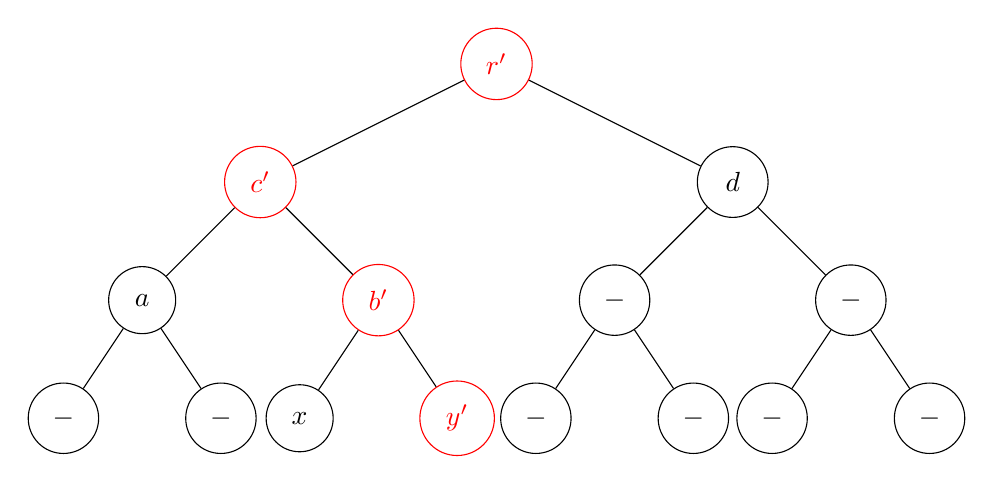
\begin{tikzpicture}[level/.style={sibling distance=60mm/#1, align=center, text centered}]
\node [circle,red,draw, text width = 1.5em, text centered] (z){$r'$}
  child {node [circle,red,draw, text width = 1.5em] (a) {$c'$}
    child {node [circle,draw, text width = 1.5em] (b) {$a$}
      child {node [circle,draw, text width = 1.5em] (c) {$-$}} 
      child {node [circle,draw, text width = 1.5em] (d) {$-$}}
    }
    child {node [circle,red,draw, text width = 1.5em] (e) {$b'$}
      child {node [circle,draw, text width = 1.5em] (f) {$x$}}
      child {node [circle,red,draw, text width = 1.5em] (g) {$y'$}}
    }
  }
  child {node [circle,draw, text width = 1.5em] (i) {$d$}
    child {node [circle,draw, text width = 1.5em] (j) {$-$}
      child {node [circle,draw, text width = 1.5em] (k) {$-$}}
      child {node [circle,draw, text width = 1.5em] (l) {$-$}}
    }
    child {node [circle,draw, text width = 1.5em] (m) {$-$}
      child {node [circle,draw, text width = 1.5em] (n) {$-$}}
      child {node [circle,draw, text width = 1.5em] (o) {$-$}}
    }
  };
\end{tikzpicture}
\caption{Incremental Computing, the updated nodes when a leaf changes \label{fig:incUp}}
\end{figure}

\subsection{Incremental Computing}
To be incremental means that, whenever some part of the data to the algorithm
changes the algorithm tries to save time by only recomputing the changed data
and the parts that depend on this changed data. \cite{incrementalDef}

For a divide and conquer lexer this would mean only recompute the changed token
and the token to the right of the changed token. This is done recurrsivly until
the root of the tree is reached. The expected result of this would be that when
a character is added to the code of 1024 tokens, instead of relex all 1024
tokens the lexer will only do 10 recalculations for new tokens. Since,
$log_2 1024 = 10$. This can be explained by the \cref{MasterTheo}. How this is
calculated for an incremental divide and conquer lexer is described more in
detail in the next sub-section.

\subsection{Expected Time Complexity}
Since incremental computing stated that only content which depends on the new
data will be recalculated. That is, follow the branch of the tree from the new
leaf to the root and recalculated every node on this path. 
As shown by \cref{fig:incUp}. Only one subproblem is updated in every level of
the tree. Back to the master theorem. Let put this in to numbers, $e = log_b a$
where $a$ is number of recursive calls and $n/b$ is size of the subproblem where
$n$ is the size of the original problem. As shown by the \cref{fig:incUp} number
of needed update calls is $1$, therefor $a = 1$. The constant $b$ is still $2$.
This will give $e = log_2 1 = 0$. Thus the update function of the incremental
algorithm will have a time complexity of
$\Theta(n^0 \cdot log n) = \Theta(log n)$

\subsubsection{The Bankers Method}
The bankers method accounts for accumulated debt. Each debit represents
a constant amount of suspended work. When a computation initially suspends, it
create a number of debits proportional to it's shared cost and
associate each debit with a location in the object. The choice of location for
each debit depends on the nature of the computation. If the computation is
monolithic (i.e., once begun, it runs to completion), then all debits are
usually assigned to the root of the result, which the incremental lexer is not. 
But if the computation is like the lexer a incremental, then the debits may be 
distributed among the roots of the partial results.

The amortized cost of an operation is the unshared cost of the operation
plus the number of debits discharged by the operation. Note that the number
of debits created by an operation is not included in its amortized cost. The
order in which debits should be discharged depends on how the object will
be accessed; debits on nodes likely to be accessed soon should be discharged
first.

Incremental functions play an important role in the bankers method because
they allow debits to be dispersed to different locations in a data structure,
each corresponding to a nested suspension. Then, each location can be accessed
as soon as its debits are discharged, without waiting for the debits at other
locations to be discharged. This means that the initial partial results of
an incremental computation can be paid for very quickly, and that subsequent
partial results may be paid for as they are needed \cite{Okasaki1999}.

\subsubsection{Banker Method on the Fingertree}
The argument for the amortized time can be expressed using the Banker method.
This is done by assigning the suspension of the middle tree in each Deep node
as many debits as the node has safe digits. (0,1 or 2) A double-ended queue
operation which descends $k$ levels turns $k$ dangerous digits into safe digits.
By doing so creates $k$ debits to pay for the work done.
Applying the bankers method of debit passing to any debits already attached to
these $k$ nodes. It can be showed that each operation must discharge at most
one debit. Therefore the double-ended queue operations run in $\Theta(1)$
amortized time \cite{fingertree}.

\section{Lexical Errors}
Since the lexer has to be able to handle any kind of possible not "complete"
tokens, error handling can be done in different ways. One approach is to simply
return as many tokens as possible from the code and where there might be lexical
errors the lexer returns the error in as small parts as possible.

\begin{example}[A lexer that only lexes letters] When the lexer encounters the
string "what @ day" it would return:
\begin{center}
\begin{tabular}{ll}
String & Type\\
What & $Word$\\
'\_' & $Space$\\
'@' & $No\_Token$\\
'\_' & $Space$\\
day & $Word$\\
\end{tabular}
\end{center}
\end{example}
